\documentclass[11pt, a4paper]{report}

\usepackage{graphicx}
\graphicspath{ {images/} }
\usepackage{caption}
\usepackage{subcaption}

\usepackage{hyperref}
\usepackage[xindy]{glossaries}
\makeglossaries
\makeindex

\usepackage[utf8]{inputenc}
\usepackage{csquotes}

\usepackage[square,sort,comma,numbers]{natbib}
\bibliographystyle{IEEEtran}

\usepackage{amsmath}
\newcommand\addtag{\refstepcounter{equation}\tag{\theequation}}
\usepackage{txfonts}

\setlength{\parindent}{0ex}
\setlength{\parskip}{1ex}

%Rechtangle painting
\usepackage{tikz}

\begin{document}
\begin{titlepage}
    \title{IP6 - Report Street Networks}
    \date{\today}
    \author{J. Peyer, S. Merki}
    \maketitle
\end{titlepage}
\setcounter{page}{1}

\tableofcontents



\begin{abstract}
    Text here.
\end{abstract}

\chapter{Introduction}

\chapter{Theoretical Task}
\section{Shape Grammar}
The main key of shape grammar is to generate networks and paintings by a new defined grammar based on shape rules, selection rules, painting rules and limiting shapes. Shape grammar is a language based on an alphabet of shapes and generated shapes \citep{shapeGrammars:1972}. 

A class of paintings defines the pair (S,M). S represents the Shape specifications and M the material specifications. The Shape specification contains "a shape grammar\ref{Shape_Grammar}, defining a language of two dimensional shapes\ref{Shape_Grammar_VT}\ref{Shape_Grammar_VM}, and a selection rule" \citep{shapeGrammars:1972}. M specifies a finite list of material specifications and one limiting shape on a canvas.

\subsection{Shape Specification\citep{shapeGrammars:1972}}
\subsubsection{Shape Grammar}
\begin{align}
\label{eq:Shape_Grammar}
SG1 &= <V_T, V_M, R, I>  \\
\label{eq:Shape_Grammar_VT}
V_T &= \{-\}  \\
\label{eq:Shape_Grammar_VM}
V_M &= \{
\includegraphics{sg_specification_VM.jpg} \}\ \\
\label{eq:Shape_Grammar_R}
R &= Rules\ R\ in\ image\ \ref{fig:Shape Grammars/Shape Specification/Rules_R} \\
\label{eq:Shape_Grammar_I}
I &= Initial\ Shape\ I\ in\ image\ \ref{fig:Shape Grammars/Shape Specification/Rules_I}
\end{align}
\subsubsection{Selection Rule}
\begin{equation}
<0,2>
\end{equation}

\begin{figure}
    \centering
    \begin{subfigure}[b]{0.3\textwidth}
        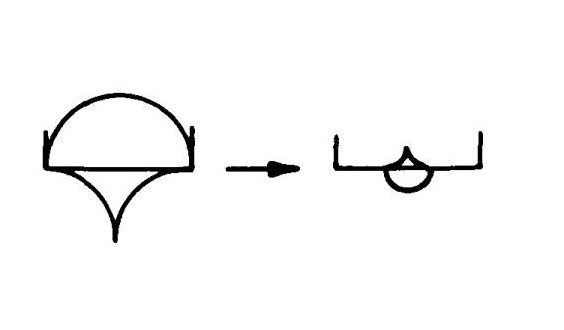
\includegraphics[width=\textwidth]{sg_specification_rule1.jpg}
        \caption{Rule 1}
        \label{fig:Shape Grammars/Shape Specification/Rule 1}
    \end{subfigure}
    ~ %add desired spacing between images, e. g. ~, \quad, \qquad, \hfill etc. 
    %(or a blank line to force the subfigure onto a new line)
    \begin{subfigure}[b]{0.3\textwidth}
        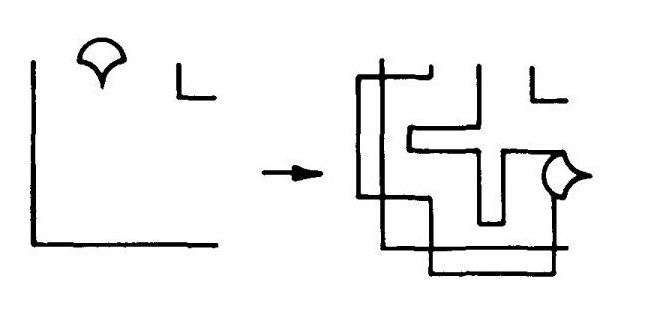
\includegraphics[width=\textwidth]{sg_specification_rule2.jpg}
        \caption{Rule 2}
        \label{fig:Shape Grammars/Shape Specification/Rule 2}
    \end{subfigure}
    ~ %add desired spacing between images, e. g. ~, \quad, \qquad, \hfill etc. 
    %(or a blank line to force the subfigure onto a new line)
    \begin{subfigure}[b]{0.3\textwidth}
        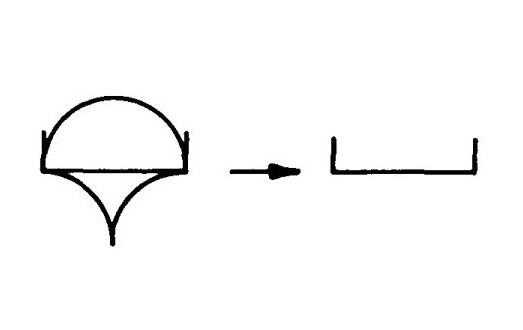
\includegraphics[width=\textwidth]{sg_specification_rule3.jpg}
        \caption{Rule 3}
        \label{fig:Shape Grammars/Shape Specification/Rule 3}
    \end{subfigure}
    \caption{ Rules R \citep{shapeGrammars:1972}}\label{fig:Shape Grammars/Shape Specification/Rules_R}
\end{figure}
\begin{figure}
    \centering
    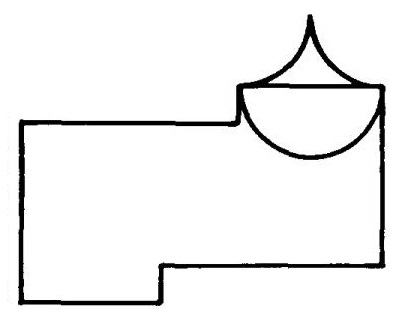
\includegraphics[width=2cm]{sg_specification_I.jpg}
    \caption{ Initial Shape I \citep{shapeGrammars:1972}}\label{fig:Shape Grammars/Shape Specification/Rules_I}
\end{figure}

\subsection{Material Specification\citep{shapeGrammars:1972}}
\subsubsection{Painting Rules}
\begin{equation}
\label{fig:Shape Grammars/Shape Specification/Painting_Rule_1}
L0\cap L1\cap L2 \Longrightarrow  
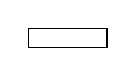
\begin{tikzpicture}
\filldraw[fill=black!00!white, draw=black] (0,0) rectangle (1,0.25);
\end{tikzpicture}
\end{equation}
\begin{equation}
\label{fig:Shape Grammars/Shape Specification/Painting_Rule_2}
(L0\cap L1\cap \sim L2)\cup (L0\cap \sim L1\cap L2)\cup (\sim L0\cap L1 \cap L2) \Longrightarrow  
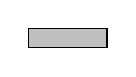
\begin{tikzpicture}
\filldraw[fill=black!25!white, draw=black] (0,0) rectangle (1,0.25);
\end{tikzpicture}
\end{equation}
\begin{equation}
\label{fig:Shape Grammars/Shape Specification/Painting_Rule_3}
(L0\cap \sim L1\cap \sim L2)\cup (\sim L0\cap L1\cap \sim l2)\cup (\sim L0\cap \sim L1 \cap L2) \Longrightarrow  
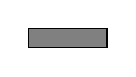
\begin{tikzpicture}
\filldraw[fill=black!50!white, draw=black] (0,0) rectangle (1,0.25);
\end{tikzpicture}
\end{equation}
\begin{equation}
\label{fig:Shape Grammars/Shape Specification/Painting_Rule_4}
\sim (L0\cup L1\cup L2)  \Longrightarrow  

\begin{tikzpicture}
\filldraw[fill=black!100!white, draw=black] (0,0) rectangle (1,0.25);
\end{tikzpicture}
\end{equation}
\subsubsection{Limiting Shape}
\begin{figure}
    \centering
    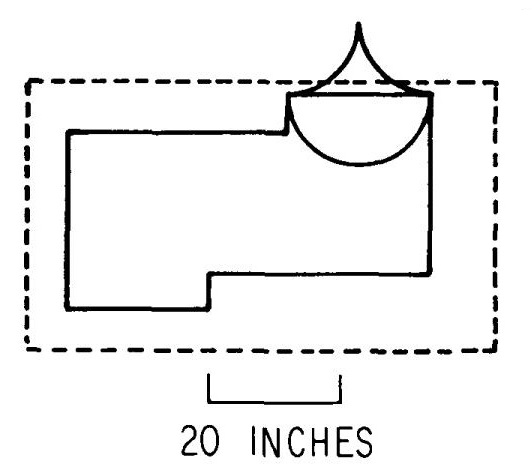
\includegraphics[width=2cm]{sg_specification_Limiting_shape.jpg}
    \caption{ Initial Shape I \citep{shapeGrammars:1972}}\label{fig:Shape Grammars/Shape Specification/Limiting_Shape}
\end{figure}
\pagebreak
\subsection{Shape Grammar Definition}
Shape Grammar is defined over an alphabet of shapes and generated n-dimensional shapes\citep{shapeGrammars:1972}.
\begin{displayquote} 
    Definition. A shape grammar (SG) is a 4-tuple: $SG = (V_T, V_M, R, I)$ where
    \begin{enumerate}
        \item $V_T$ is a finite set of shapes.
        \item $V_M$ is a finite set of shapes such that $V_T $* $\cap$  $V_M = \emptyset$
        \item R is a finite set of ordered pairs (u.v) such that u is a shape consisting of an element of $V_T $* combined with an element of $V_M$ and v is a shape consisting of (A) the element of $V_T $* contained in u or (B) the element of $V_T $* contained in u combined with an element of $V_M$ or (C) the element of $V_T $* contained in u with an additional element of $V_T$* and an element of $V_M$.
        \item I is a shape consisting of elements of $V_T $* and $V_M$.
    \end{enumerate}
\end{displayquote}
$V_T $* 
The following image describes the generative specifications and some examples rules.
\pagebreak


\subsection{Shape Rules}
A shape rule is de definition what should be painted based on the current state of the painting. The Initial Shape has not to be inside of the Limiting Shapes.

\pagebreak
\subsection{Selection Rules}
An undefined count of shape rules provide the generation of the painting. Therefore a mechanism to select a correct shape is required. The depth is defined by levels. Like the authors G. Stiny and J. Gips describe in "Shape Grammars and the Generative Specification of Painting and Sculpture  \citep{shapeGrammars:1972}.
\begin{displayquote}
    Level assignments are made to terminals during the generation of a shape using these rules:
    \begin{enumerate}
        \item The terminals in the initial shape are assigned level 0.
        \item If a shape rule is applied, and the highest level assigned to any part ot the terminal corresponding to the level side of the rule is N, then
        \begin{enumerate}
            \item If the rule is of type A, any part of the terminal enclosed by the marker in the left side of the rule is assigned N.
            \item If the rule is of type B, any part of the terminal enclosed by the marker in the left side of the rule is assigned N and any part of the terminal enclosed by the marker is assigned N + 1.
            \item If the rule is of type C, the terminal added is assigned N + 1.
        \end{enumerate}
        \item No other level assignments are made.
    \end{enumerate}
\end{displayquote}

\subsection{Painting Rules}
Painting rules describe witch shape should be painted inside of a defined area. Like in a Venn diagram the rules contain multiple levels 0 - n. By combining this levels the painting colour is described. As describes in more details by the authors G. Stiny and J. Gips in "Shape Grammars and the Generative Specification of Painting and Sculpture \citep{shapeGrammars:1972}.
\begin{displayquote}
    Painting rules indicate how the areas contained in a shape painted by considering the shape as a Venn diagram as in naive set theory. The terminals of each level in a shape are taken as the outline of a set in the Venn diagram. As parts ot terminals may be assigned multiple levels, sets may have common boundaries. Levels 0, 1, 2, ..., n are said to define sets L0, L1, L2, ..., Ln respectively where n is given in the selection rule.
    \newline
    A painting rule has two sides separated by a double arrow ($\Rightarrow$). The left side of a painting rule defines a set using the sets determined by level assignment and the usual set operators, for example, union($\bigcap$), intersection ($\bigcup$), complementation($\sim$), and exclusive or ($\bigotimes$), The sets defined by the left side of the painting rules of M must partition the universal set. The right side of a painting rule is a rectangle painted in the manner the set defined by the left side of the rule is to be painted.
\end{displayquote}

\subsection{Limiting Shapes}
These Shapes define a limiting area on the canvas, where shape painting is allowed. 
The area could have any form, but normally it is defined as a rectangle. Like a camera view the Limiting Shape define the scale of a painting and its viewpoint. Therefore the initial/start shape could be outside of the limiting shape 



\pagebreak
\section{Procedural Modelling}

\pagebreak
\section{L-Systems}

L-System is a well established modelling approach for the synthesis of realistic plant images. There are many papers describing L-Systems and how they are applied to generate plant live: [TODO: reference those papers] "In these cases L-System productions capture the \textit{development} of plant components over time." \citep{PrusinkiewiczEtAl:2001} Productions are applied in parallel, so that all plant parts grow and age equally. The growth is stopped at a defined terminal age. This age is the number of iterations, where in each iteration productions are applied.
\subsection{TODO: reference papers here}
The context-free productions in \citep{PrusinkiewiczEtAl:2001} are defined using the following syntax.
\begin{equation} \label{lsystem context free}
    pred : \{block1\}\ cond\ \{block2\} \leadsto succ
\end{equation}
The symbol \textit{pred} (predecessor) defines the module that will get replaced by the modules defined in \textit{succ} (successor). This replacement is only applied, if the (optional) condition is met. \textit{block1} and \textit{block2} are C statement blocks, of which the first block is executed before and the second after the condition is evaluated. \citep{PrusinkiewiczEtAl:2001} gives the following example.
\begin{equation} \label{lsystem example 1}
    A(x) : \{y = x + 2;\}\ y \geq 5\ \{z = y / 3;\}\ \leadsto B(z)C(z + 1)
\end{equation}
If this example production was applied to the module $A(4)$, it would result in the modules $B(2)C(3)$.

The cpfg language, described in \citep{PrusinkiewiczEtAl:2001}, also supports context-sensitive productions. The following listing defines the syntax of such a production.
\begin{equation} \label{lsystem context sensitive}
    lcont < pred > rcont : \{block1\}\ cond\ \{block2\} \leadsto succ
\end{equation}
\textit{lcont} (left context) and \textit{rcont} (right context) each define a list of modules that have to precede or respectively follow the \textit{pred} (module being replaced). Context modules are limited to query symbols, which are explained later on. \citep{PrusinkiewiczEtAl:2001} gives the following example.
\begin{equation} \label{lsystem example 2}
    A(x) < B(y) > C(z) : x + z > 0 \leadsto M(y / 2)N(y / 2)
\end{equation}
If the example of listing \ref{lsystem example 2} was applied to the module composition $A(2)B(4)C(0)$, it would result in the modules $A(2)M(2)N(2)C(0)$.

\pagebreak
\section{Chomsky Grammars?}
\citep{PrusinkiewiczEtAl:2001}
Almost like L-System but with minor modifications.

\pagebreak
\chapter{Practical Task}
\section{CPlan}
\subsection{Changes}
\begin{itemize}
    \item The function .toArray() creates a complete copy of the existing enumeration in the ram. Therefore the application had an extremely large footprint. To reduce the coping we changed some methods to be called directly with IEnumerable Parameters.
    \item If some extension methods are created the should be tested by unit tests.
\end{itemize}


\subsection{New Functions}
\subsubsection{Graph to Tree}


\chapter{Conclusion}

\bibliography{quotations}
\appendix
\glsaddall
\printglossaries
\end{document}